% =============================================================================
%  Section 2.3 — Các hệ thống sinh tăng cường truy hồi
% =============================================================================

\section{Các hệ thống sinh tăng cường truy hồi }
\subsection{Phương pháp tạo sinh tăng cường truy hồi truyền thống - RAG}

Retrieval-Augmented Generation (RAG) \cite{lewis2020rag} là kiến trúc kết hợp giữa mô hình truy hồi thông tin và mô hình sinh ngôn ngữ nhằm nâng cao độ chính xác của câu trả lời. Thay vì để mô hình ngôn ngữ sinh nội dung hoàn toàn dựa trên tập dữ liệu mà nó được huấn luyện, hệ thống RAG thực hiện truy vấn từ một kho dữ liệu bên ngoài để tìm các đoạn văn bản liên quan đến câu hỏi. Các đoạn văn bản này sau đó được đưa vào prompt làm ngữ cảnh bổ sung, từ đó giúp mô hình đưa ra câu trả lời dựa trên thông tin cụ thể hơn. Cách tiếp cận này cho phép hệ thống khai thác hệ thống tri thức được cập nhật liên tục và giảm nguy cơ tạo ra nội dung sai lệch.

Trong kiến trúc RAG truyền thống (Hình \ref{fig:overviewRAG}), quy trình thường bao gồm các bước: mã hóa câu hỏi thành dạng vector, tìm kiếm các đoạn văn bản có độ tương đồng cao trong cơ sở dữ liệu vector (tương đồng về mặt ngữ nghĩa), và kết hợp các đoạn này vào prompt trước khi gửi đến mô hình ngôn ngữ. Phương pháp này có ưu điểm là không yêu cầu huấn luyện lại mô hình và có thể dễ dàng tích hợp với các cơ sở dữ liệu mới. Tuy nhiên, RAG truyền thống chủ yếu dựa trên độ tương đồng ngữ nghĩa giữa các đoạn văn bản, do đó việc truy hồi phụ thuộc mạnh vào chiến lược chia nhỏ văn bản (chunking) và chất lượng mã hóa (embedding).

\begin{figure}
    \centering
    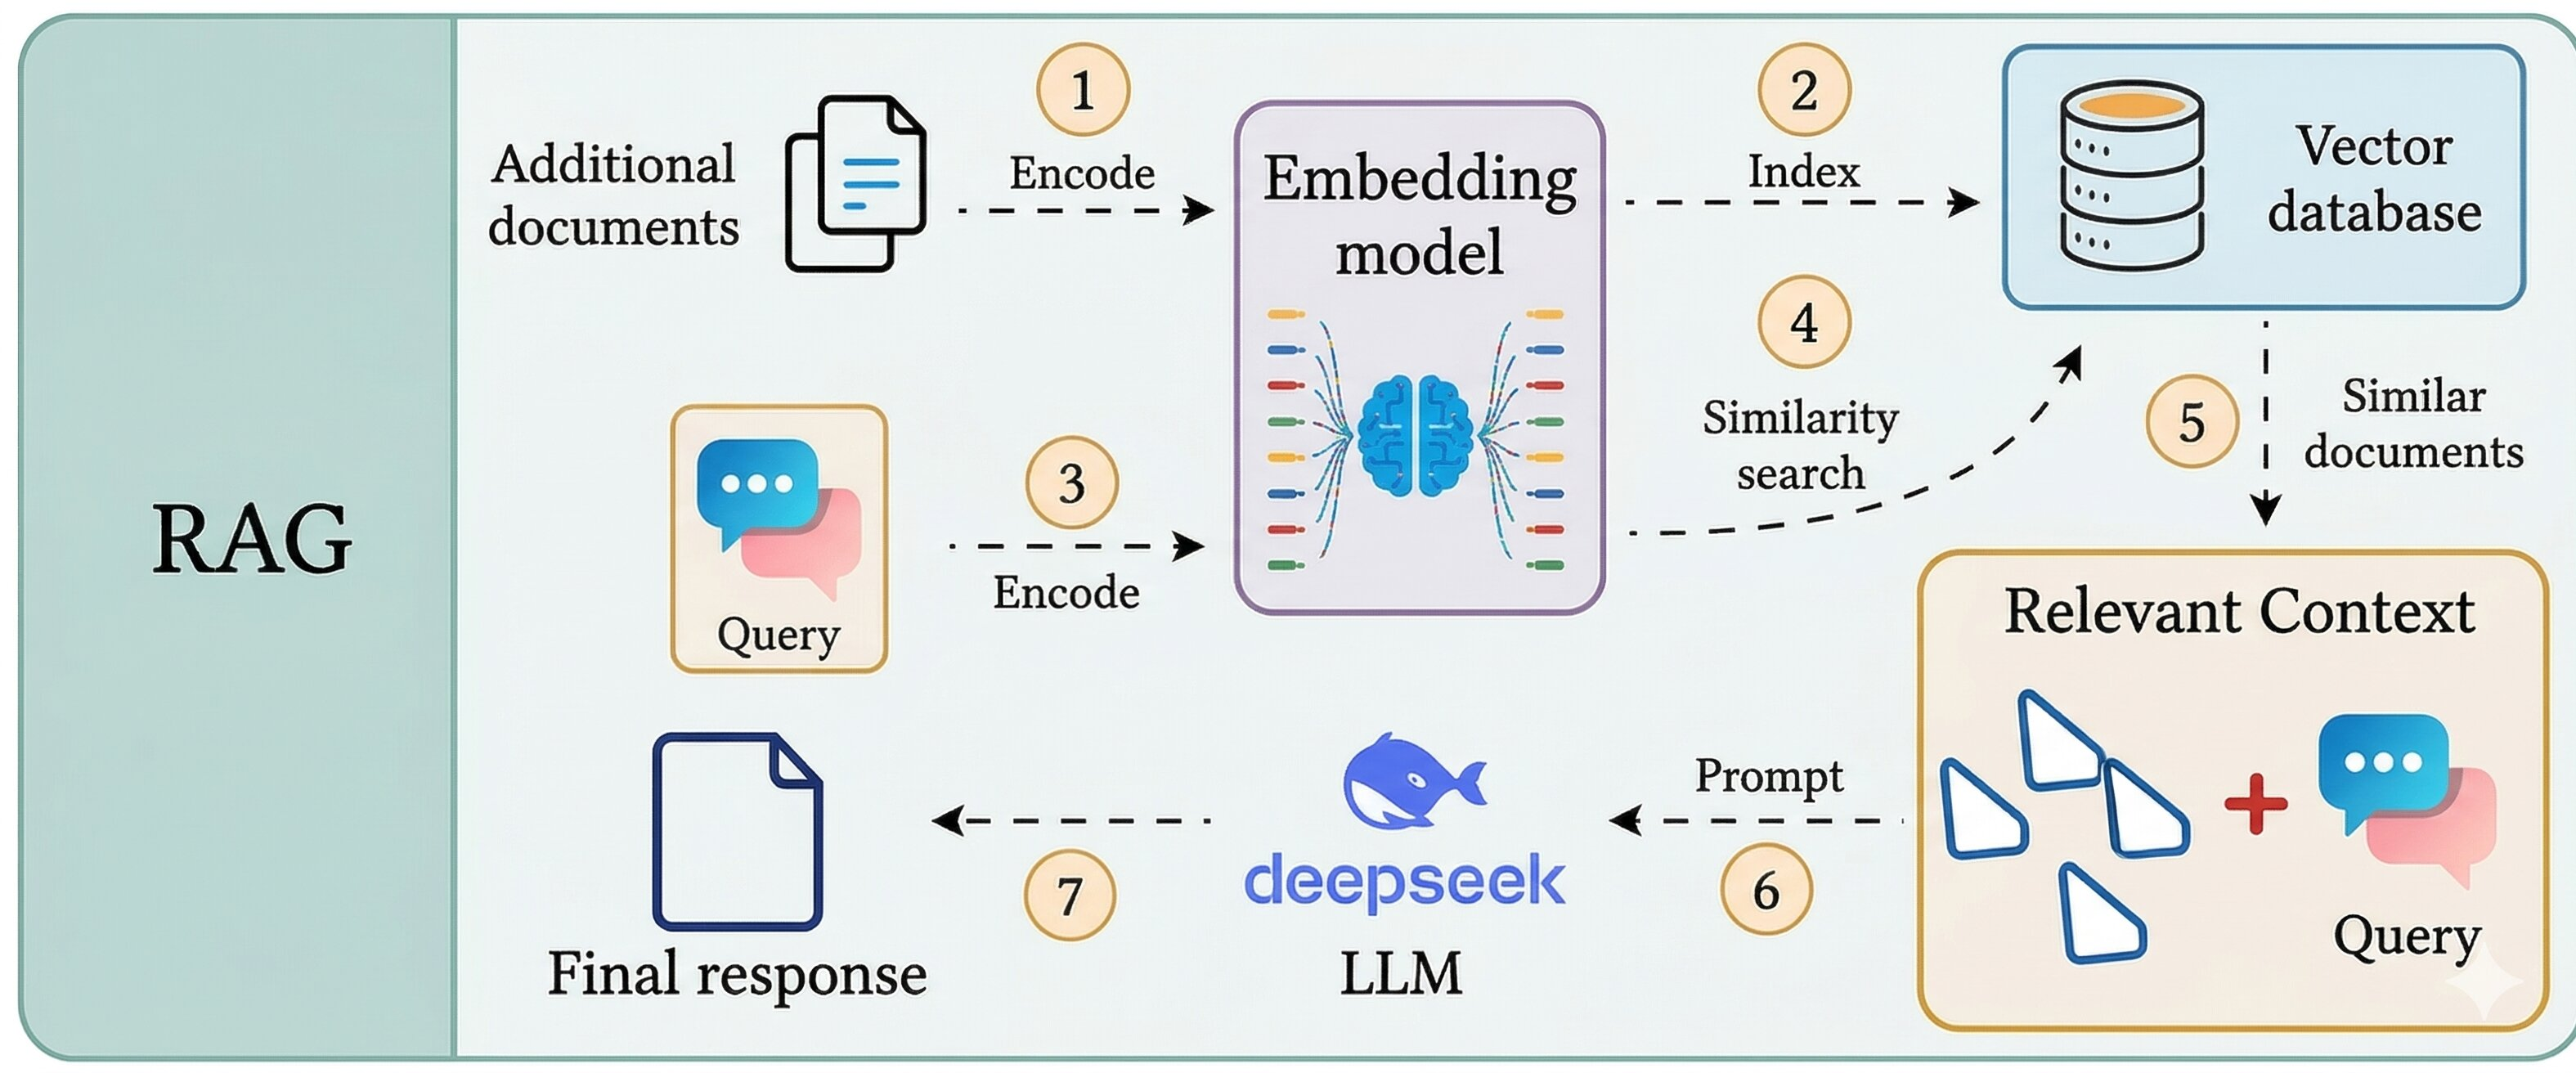
\includegraphics[width=0.9\linewidth]{figures//c2/RAG.jpg}
    \caption{Tổng quan kiến trúc RAG}
    \label{fig:overviewRAG}
\end{figure}

Một hạn chế cốt lõi của RAG truyền thống là thiếu khả năng khai thác cấu trúc quan hệ giữa các thực thể. Khi câu hỏi yêu cầu tổng hợp thông tin từ nhiều nguồn hoặc yêu cầu suy luận đa bước, việc chỉ truy hồi các đoạn văn bản rời rạc có thể không cung cấp đủ ngữ cảnh cần thiết. Ngoài ra, RAG khó đảm bảo rằng các đoạn văn bản được truy hồi có mối liên hệ logic chặt chẽ với nhau, bởi cơ chế truy hồi chủ yếu dựa trên mức tương đồng ngữ nghĩa. Chính những hạn chế này đã thúc đẩy sự phát triển của các phương pháp tích hợp tri thức có cấu trúc hơn, trong đó GraphRAG là một hướng tiếp cận tiêu biểu.

\subsection{Phương pháp tạo sinh tăng cường truy hồi dựa trên đồ thị - GraphRAG}

GraphRAG \cite{gong2025triplet,zhu2025kgguidedrag,hu2025grag} là một mở rộng của kiến trúc RAG, thay vì làm việc với cơ sở dữ liệu với hàng triệu bản ghi dạng chữ, dạng bảng thì nó làm việc với cơ sở tri thức là đồ thị tri thức. Trong đó tầng truy hồi thông tin không chỉ dựa trên độ tương đồng ngữ nghĩa mà còn khai thác cấu trúc quan hệ đang tồn tại của đồ thị tri thức. Thay vì truy hồi các đoạn văn bản độc lập, hệ thống có thể truy xuất các thực thể và quan hệ liên quan trong đồ thị tri thức (Hình \ref{fig:overview_graphrag}), từ đó xây dựng mạng lưới thông tin phù hợp với truy vấn. Mạng lưới thông tin này sau đó được chuyển đổi thành dạng ngữ cảnh văn bản hoặc biểu diễn có cấu trúc để cung cấp cho mô hình ngôn ngữ. Nhờ đó, quá trình sinh câu trả lời được định hướng bởi cấu trúc quan hệ thay vì chỉ dựa vào độ tương đồng ngữ nghĩa thông qua mã hóa thông tin.

\begin{figure}
    \centering
    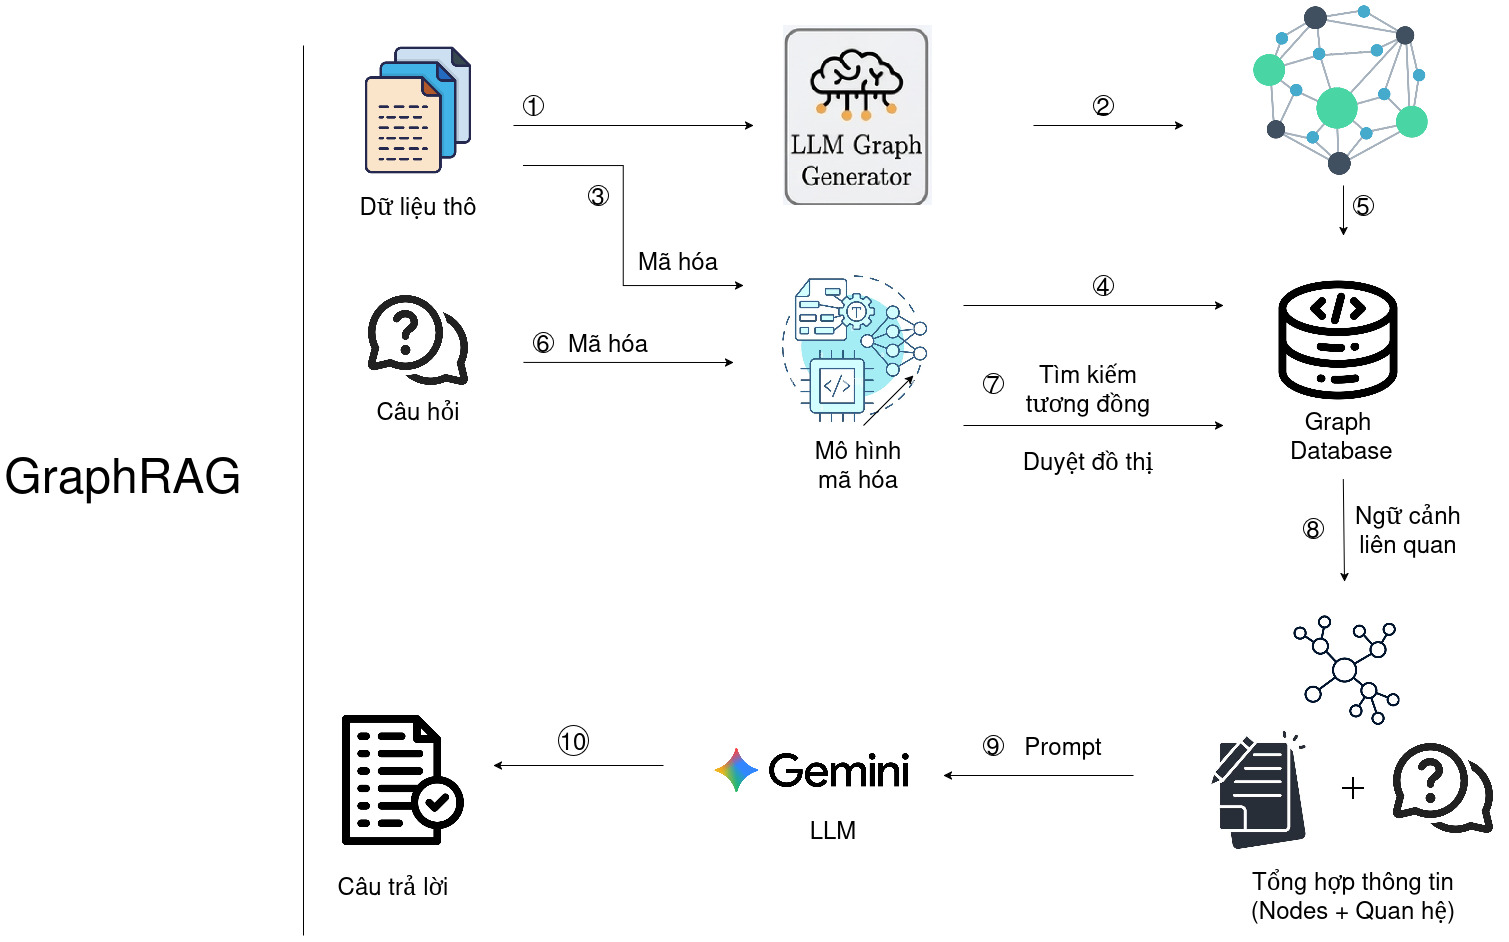
\includegraphics[width=0.9\linewidth]{figures//c2/GraphRAG.jpg}
    \caption{Tổng quan kiến trúc GraphRAG}
    \label{fig:overview_graphrag}
\end{figure}

Điểm khác biệt quan trọng giữa RAG truyền thống và GraphRAG nằm ở khả năng hỗ trợ suy luận đa bước. Trong khi RAG chủ yếu truy hồi các đoạn văn bản có liên quan trực tiếp đến câu hỏi, GraphRAG có thể mở rộng truy vấn thông qua các cạnh trong đồ thị để khám phá các thực thể liên quan gián tiếp. Với khả năng này, GraphRAG có thể trả lời được các câu hỏi yêu cầu tổng hợp thông tin từ nhiều nguồn hoặc yêu cầu phân tích mối quan hệ giữa các thực thể. Đồ thị tri thức được xây dựng kĩ lưỡng sẽ giúp đảm bảo rằng ngữ cảnh được cung cấp cho mô hình có tính liên kết logic, thay vì là tập hợp các đoạn văn bản rời rạc. Đồng thời, các câu trả lời của GraphRAG có mức tin cậy cao nhờ việc xây dựng từng đồ thị con với từng câu hỏi, mỗi câu trả lời có thể được truy vết thông qua chuỗi quan hệ giữa các thực thể trong đồ thị tri thức.

Trong phạm vi nghiên cứu này, GraphRAG được sử dụng như một cơ chế tổ chức và cung cấp tri thức có cấu trúc cho hệ thống trả lời câu hỏi. Mô hình ngôn ngữ đóng vai trò thành phần sinh câu trả lời, trong khi đồ thị tri thức đảm nhiệm việc điều hướng và mở rộng ngữ cảnh dựa trên quan hệ thực thể. Sự kết hợp này cho phép tận dụng khả năng sinh ngôn ngữ của mô hình đồng thời khai thác cấu trúc tri thức của đồ thị.
